\documentclass[a4paper, twopage]{scrreprt}

\usepackage[ngerman]{babel}
\usepackage[utf8]{inputenc}
\usepackage[backend=bibtex, style=numeric]{biblatex}
\usepackage{hyperref}
\usepackage{graphicx}

\author{Samuel Hammer}
\title{Vorgehensmodelle zur Projektentwicklung}
\subtitle{Ausarbeitung für die mündl. PRE Matura 2015}

\bibliography{quellen.bib}

\begin{document}

\maketitle
\tableofcontents

\chapter{Einleitung}
\label{ch:einleitung}
IT-Projekte können je nach konkretem Anwendungsfall unterschiedlich groß bzw. komplex werden. Um unabhängig von diesen Faktoren die Übersichtlichkeit, Organisation und Struktur eines Projektes zu gewährleisten, gibt es verschiedene Vorgehensmodelle. \newline
Die existierenden Vorgehensmodelle lassen sich grob in zwei Kategorien unterteilen: 
\begin{itemize}
	\item Klassische Phasenmodelle
	\item Vorgehensmodelle zur agilen Softwareentwicklung
\end{itemize}
Abhängig vom Anwendungsfall, können verscheidene Vorgehensmodelle verschiedene Vor- und Nachteile für das Projekt haben. In der Praxis gibt es also in den seltensten Fällen ein Modell, das für die Durchführung des Projektes hundertprozentig passt.
\begin{figure}[h]
\centering
	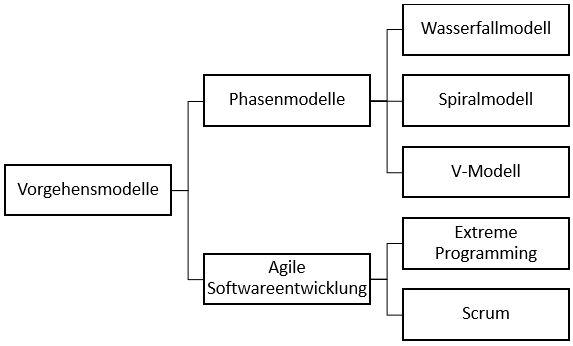
\includegraphics[scale=0.6]{Images/vorgehensmodelle_diagramm}
	\caption{Übersicht über Vorgehensmodelle\label{fig:vorgehensmodelle_diagramm}}
\end{figure}

\newpage

\section{Phasenmodelle}
\label{sec:phasenmodelle}
Phasenmodelle sind "standardisierte Projektstruckturen für die Erstellung des Projektprodukts". \footnote{\cite{wikipedia:projektphase}}
Da allerdings nicht auf jedes Projekt die selben Phasen zutreffen, gibt es verschieden Abwandlungen. Für Softwareprojekte wird in der Regel folgende Phasenstruktur verwendet:
\begin{enumerate}
	\item Anforderungen
	\item Analyse
	\item Design
	\item Entwicklung
	\item Test
\end{enumerate}
Wenn diese verschiedenen Phasen des Projektes komplett sequentiell und unabhängig voneinander stattfinden, so spricht man vom klassischen Wasserfallmodell. (Siehe Kapitel \ref{ch:wasserfallmodell}
In der Praxis hat sich das strikte vorgehen von oben nach unten (also wie ein Wasserfall) allerdings nicht bewährt, da dieses Modell es nicht erlaubt einzelne Phasen zu wiederholen.
Für diesen Fall wurden iterative Modelle entwickelt. Hier können dann einzelne Phasen wiederholt werden falls sich beispielsweise während des Projektes die Anforderungen verändern.
\section{Agile Softwareentwicklung}
\label{sec:agile_softwareentwicklung}
Agile Softwareentwicklung gibt es seit den frühen 1990er Jahren. Mit steigender komplexität der Softwareprojekte, wurde auch der Aufwand in Bezug auf das Projektmanagement immer größer. Da klassische Phasenmodelle aufgrund ihrer geringen Flexibilität nicht mehr praktikabel waren, wurde das sogenannte "Agile Manifest" verfasst. Das Agile Manifest ist ein Werk, in dem Agile Werte definiert werden, um Softwareprojekte einfacher und besser zu gestalten. Ein Auszug aus dem Agilen Manifest besagt: \paragraph*{}
"Wir erschließen bessere Wege, Software zu entwickeln, indem wir es selbst tun und anderen dabei helfen. Durch diese Tätigkeit haben wir diese Werte zu schätzen gelernt:
\begin{itemize}
	\item \textbf{Menschen und Interaktionen} mehr als Prozesse und Werkzeuge
	\item \textbf{Funktionierende Software} mehr als umfassende Dokumentation
	\item \textbf{Zusammenarbeit mit dem Kunden} mehr als Vertragsverhandlung
	\item \textbf{Reagieren auf Veränderung} mehr als das Befolgen eines Plans
\end{itemize}
Das heißt, obwohl wir die Werte auf der rechten Seite wichtig finden, schätzen wir die Werte auf der linken Seite höher ein.“ \footnote{\cite{agilemanifesto}}

\chapter{Wasserfallmodell}
\label{ch:wasserfallmodell}


\chapter{Inkrementalmodell}

\chapter{Evolutionsmodelle}

\section{Rapid Prototyping}

\chapter{Spiralmodell}


\nocite{*}
\printbibliography

\listoffigures

\end{document}